\section{Methodology}

The purpose of this research is to catalog code smells of the Android presentation layer. Thus, we conducted a mixed study~\cite{CreswellResearch:13}. According to research~\cite{arcverde2011understanding, Palomba_Do_2014, yamashita2013developers}, empirical perception plays an important role in the definition of code smells related to a specific technology, especially considering their intrinsic subjective nature~\cite{JavascriptSmells, JavaQADetectingSmells:02}.

Our mixed approach comes in such a way that the code smells are collected by means of two online questionnaires, answered by 246 Android developers. We then performed an online code experiment about the perceptions of developers on the proposed smells, where we obtained 70 responses. 

We explain the three parts of this research in the following sub-sections.

\subsection{Part 1 - Best and bad practices in the presentation layers of Android apps}
\label{etapa-1}

The goal of this part was to collect the best and the bad programming practices 
that developers perceive when developing the presentation layer of Android apps.
To that aim, we devised an online questionnaire composed of exploratory questions
about each one of the components in Android's presentation layer 
(\textit{Activities}, \textit{Fragments}, \textit{Adapters}, \textit{Listeners}) 
as well as application resources (\textit{Layout}, \textit{Strings}, 
\textit{Styles} and \textit{Drawables}). 

\subsubsection{Questionnaire}
\label{etapa-1-questionario}

This questionnaire was based on an earlier study by Aniche et al.~\cite{AnicheSmellsMVC:17, FinavaroAniche2016}, where authors searched for code smells in \acs{MVC} applications. 
We informed participants that this was part of a research on Android code quality and that the data provided would be published anonymously. The questionnaire was composed of 25 separate questions in three sections.

The first section had the goal of tracing the participant's demographic profile (age, state of residence, experience in software development, experience with Android development and schooling) and was composed of 6 questions. The second section aimed at understanding what developers considered best and bad practices in the development of the Android presentation layer. It consisted of 16 optional and open questions, 8 on best practices for each of the 8 elements of the Android presentation layer, and 8 on bad practices. The complete questionnaire can be seen in Appendix~\ref{ap: survey-1}. 
For example, for the \textit{Activity} element, the second section contained the following questions:

\begin{itemize}
  \item[Q1] Do you have any good practices to deal with Activities? (Open question)
  \item[Q2] Do you have anything you consider a bad practice when dealing with Activities? (Open question)
\end{itemize}


The third section consisted of three optional open questions, 
two to capture any last ideas that we did not capture in the previous questions, and one requesting the participant's email, if he or she had an interest in participating in future research steps.

Before the release, we conducted a pilot test with three Android developers. In the first configuration of the questionnaire, all questions, from all sections except email, were mandatory. With the result of the pilot test, we realized that developers not always have some best or bad practice to comment on all components. Thus, we made such questions optional. Responses from pilot participants were disregarded to mitigate bias effects.

The questionnaire was released on social networks like Facebook, Twitter, Slack, and LinkedIn\footnote{We will give more information about communities we share in the camera ready, as it could reveal authors' identities}. The questionnaire was open for approximately 3.5 months, from October 9, 2016 until January 18, 2017.

\subsubsection{Participants}
\label{etapa-1-participantes}

We obtained 45 responses from Android developers. 
90\% of the respondents have two years or more of software development experience, 
and 71\% have two years or more of experience with Android development. 
It is noteworthy that the Android platform completes 10 years in 2018, i.e., 
five years of experience in this platform represents 50\% of Android's lifetime
since its announcement in 2008.

\textcolor{red}{suelen: descrever os graficos aqui em palavras. apenas um paragrafo curto.}

The questionnaire was replied by professionals from 3 continents and 7 different countries.
However, most participants come from BLINDED, with a little more than 81\% of participants.
Thus, we believe that it is more appropriate to say that code smells may better reflect the opinions of BLINDED developers. In future research, we plan to collect more answers from
different regions of the globe.

\subsubsection{Data analysis}
\label{etapa-1-analise}

Our analysis process was inspired by the Ground Theory approach (GT), a research method originated in the social sciences~\cite{Strauss2007, GlaserStrauss1999}, but increasingly popular in software engineering research~\cite{Adolph2011}. 
GT is an inductive approach, whereby data from, e.g., interviews or questionnaires, are analyzed to derive a theory. The goal is to discover new perspectives rather than confirm any existing ones. The analysis process started from the list of 45 responses of the questionnaire and was given in 4 steps: \textit{verticalization}, \textit {data cleaning}, \textit {codification}, and \textit {division}, detailed below.

The process we called \textit{verticalization} consisted of considering each best or bad practice response as an individual record to be analyzed. That is, each participant answered 18 questions about good and bad practices in the Android presentation layer (2 questions for each element and 2 more generic questions). With the process of verticalization, each of these answers became a record, that is, each participant resulted in 18 answers to be analyzed, totaling 810 answers.

The next step was to perform the \textit{data cleaning}. This step consisted of removing obviously non-useful answers as blank answers, answers containing phrases like "No", "Not that I know", "I do not remember"}, the ones considered vague as \textit {"I'm not sure if they are good practices but I use what I see there"}, those considered generic as \textit{"Like all Java code ..."}, and those not related to best or bad code practices. Of the 810 answers, 352 were considered and 458 were disregarded. Of the 352, 45\% were related to bad practices, and 55\% to best practices.

Next, we performed \textit{codification} on best and bad practices~\cite{Strauss2007, Saldana2013}. Codification is the process by which categories are extracted from a set of statements through the abstraction of central ideas and relations between the statements~\ cite{Strauss2007}. During this process, each response received one or more categories. In this step we disregarded some more answers: this occurred because they were not `` obviously '' disposable responses like those of the previous step, and deeper analysis was necessary to arrive at this conclusion. For each response not considered in this step we recorded the reason, which can be checked in the files in our online appendix~\cite{apendice}.

Finally, we performed the \textit {split} step. This step consisted in dividing responses that belonged to more than one category into two or more responses.
As an example, \textit{``Do not make Activities to be callbacks of assynchronous executions. Always inherit from support classes, never directly from the platform.''} indicates in the first sentence a category and in the second sentence, another category. By dividing it, we kept only the segment of the response relative to the category, as if they were two distinct and valid answers. In some cases, the complete response was necessary to understand both categorizations, in which case we maintained the original response, even if duplicated, and categorized each one differently.

At the end of the analysis, there were 359 responses on best and bad practices individually categorized into 46 categories. 
To be considered a code smells, we collected all categories in which the number
of responses were greater than or equal to five.
According to Nielsen~\cite{NielsenMagicNumber: 00}, five repetitions is enough to obtain the data required to define a problem, and the following repetitions tend not to aggregate new relevant information. We then considered each of these categories as a code smell.
We obtained 20 code smells, of which nine are related to the components of the Android presentation layer, and 11 related to application features.

\subsection{Etapa 2 - Importância e Frequência dos Maus Cheiros Android}



Para responder a QP$_2$, buscamos generalizar os maus cheiros encontrados na QP$_1$ entendendo a percepção dos desenvolvedores com relação à frequência e importância dos maus cheiros. Coletamos esta percepção por meio de um questionário online com três seções sendo a primeira para coleta de dados demográficos da mesma forma da etapa 1, a segunda para coleta da percepção de frequência dos maus cheiros no dia a dia de desenvolvimento e a terceira para coleta da percepção de importância. 

Coletamos 201 respostas de desenvolvedores Android de 3 continentes e 14 países diferentes. Nossos resultados mostraram que os 20 maus cheiros são considerados, de algum modo, frequentes e importantes. A seguir, na Seção \ref{etapa-2-questionario} apresentamos detalhes sobre a concepção do questionário, na Seção \ref{etapa-2-participantes} detalhes sobre os participantes e na Seção \ref{etapa-2-analise} detalhes sobre o processo de análise dos dados. Os resultados desta etapa podem ser conferidos na Seção \ref{phase2-results}.

\subsubsection{Questionário}
\label{etapa-2-questionario}

Foram criadas duas versões do questionário, inglês e português, de forma que de um era possível acessar o outro, possibilitando o participante escolher o idioma mais apropriado a ele. No cabeçalho do questionário inserimos algumas informações para o participante, dentre elas, informamos que o questionário fazia parte de uma pesquisa sobre qualidade de código Android e que os dados fornecidos poderiam futuramente ser publicados de forma anônima. O questionário (S$_2$) continha 3 seções. A primeira seção, como em S$_1$, tinha o objetivo de traçar o perfil demográfico do participante (idade, estado de residência, experiência em desenvolvimento de software, experiência com desenvolvimento Android e escolaridade) e foi composta de 6 perguntas. 

A segunda seção objetivou capturar a percepção dos desenvolvedores com relação à frequência em que eles percebiam os maus cheiros no seu dia a dia. Fizemos isso apresentando uma lista de afirmações onde cada afirmação descrevia um sintoma de um dos maus cheiros. Para cada afirmação o participante podia escolher uma entre cinco opções da escala \textit{likert} de frequência: muito frequente, frequente, às vezes, raramente e nunca. 

As afirmações foram baseadas nas respostas de S$_1$, por exemplo, para o mau cheiro \textsc{\small Classes de UI Acopladas} algumas das respostas sobre más práticas foram \textit{``Acoplar o \textit{Fragment} a \textit{Activity} ao invés de utilizar interfaces é uma prática ruim''} (P19) e \textit{``Acoplar o \textit{Fragment} com a \textit{Activity}''} (P10, P31 e P45), e boa prática foi \textit{``Seja um componente de UI reutilizável. Então evite dependência de outros componentes da aplicação''} (P6). Com base nessas e outras respostas extraímos a seguinte frase para representar o sintoma do mau cheiro:

\begin{itemize}
 \item \textit{Fragments}, \textit{Adapters} ou \textit{Listeners} com referência direta para quem os usa, como \textit{Activities} ou outros \textit{Fragments}.
\end{itemize}

Para contemplar os 20 maus cheiros, foram apresentadas 25 afirmações sobre frequência. Essa diferença do número total de maus cheiros e o número de afirmações ocorreu pois, para 4 dos maus cheiros (\textsc{\small Comportamento Suspeito}, \textsc{\small Layout Longo ou Repetido}, \textsc{\small Longo Recurso de Estilo} e \textsc{\small Atributos de Estilo Repetidos}), foram apresentadas mais de uma afirmação, cada qual abordando um dos sintomas apresentados por ele. Optamos por separar os sintomas em afirmações para entender qual(is) sintoma(s) era percebido no dia a dia pelo desenvolvedor. Por exemplo, para o mau cheiro \textsc{\small Comportamento Suspeito} apresentamos três afirmações, onde cada uma representou uma forma diferente, considerada má prática pelos participantes de S$_1$, sobre como implementar a resposta a eventos do usuário no Android:

\begin{itemize}
  \item \textit{Activities}, \textit{Fragments} ou \textit{Adapters} com classes anônimas para responder a eventos do usuário, como clique, duplo clique e outros.

  \item \textit{Activities}, \textit{Fragments} ou \textit{Adapters} implementando algum \textit{Listener}, através de polimorfismo (\textit{implements}), para responder a eventos do usuário como clique, duplo clique e outros.

  \item \textit{Activities}, \textit{Fragments} ou \textit{Adapters} com classes internas implementando algum \textit{Listener} para responder a eventos do usuário como clique, duplo clique e outros.
\end{itemize}

A terceira seção objetivou capturar a percepção dos desenvolvedores com relação à importância em mitigar os sintomas dos maus cheiros, para isso foi solicitado que indicasse o quão importante ele considerava as afirmações apresentadas. Para contemplar os 20 maus cheiros, apresentamos 21 afirmações de importância que basicamente negavam as afirmações relacionada à percepção de frequência do mau cheiro. A divergência do total de maus cheiros e o total de afirmações apresentadas se dá pelo mesmo motivo encontrado na seção anterior do questionário, sobre percepção de frequência. Para cada afirmação o participante podia escolher uma dentre as cinco opções da escala \textit{likert} de importância: muito importante, importante, razoavelmente importante, pouco importante, não é importante. A seguir apresentamos a afirmação apresentada nesta seção para o mau cheiro \textsc{\small Classes de UI Acopladas}:

\begin{itemize}
  \item \textit{Fragments}, \textit{Adapters} e \textit{Listeners} não ter referência direta à quem os utiliza.
\end{itemize}

Em nenhuma das seções indicamos que seriam apresentados sintomas de maus cheiros, nem mencionamos os nomes dos maus cheiros usados nesta dissertação, foram apresentadas somente as afirmações. Optamos por fazer desta forma para abstrair a ideia de que as frases representavam maus cheiros e portanto, não exigir do participante um conhecimento prévio sobre maus cheiros de código.

Antes da divulgação do questionário realizamos a validação de cada uma das afirmações, por meio de entrevista individual, com dois desenvolvedores Android experientes, \emph{DEV-A} e \emph{DEV-B}. \emph{DEV-A} possui 10 anos de experiência com desenvolvimento de software e 5 anos de experiência com desenvolvimento Android, se considera proficiente nas tecnologias Java, Objective C, Swift e Android e possui bacharel em Tecnologia de Informação. \emph{DEV-B} possui 7 anos de experiência com desenvolvimento de software e 6 anos de experiência com desenvolvimento Android, se considera proficiente nas tecnologias Java, Objective C e Android e possui pós-graduação em Engenharia de Software Orientada a Serviços. Ambos os desenvolvedores trabalham atualmente com desenvolvimento de aplicativos móveis em \textit{startups} brasileiras. 

A entrevista de validação das afirmações foi conduzida de modo que o desenvolvedor procedia respondendo o questionário e quando tinha dúvida sobre uma frase, o mesmo questionava e então ela era discutida e quando necessário, reestruturada ou reescrita, de acordo com o comentário dado. Após a discussão, o desenvolvedor a respondia, considerando a conclusão das discussões, e seguia para a próxima. Essa dinâmica seguiu até passar por todas as afirmações e ao final o desenvolvedor era incentivado a dar qualquer outro comentário que considerasse relevante. 

Alguns importantes ajustes foram realizados após a primeira entrevista de validação. O principal ajuste foi relacionado a escala \textit{likert} utilizada, sendo que, na primeira versão do questionário, respondido por \emph{DEV-A}, foi usada tanto para validar importância quanto para validar frequência a mesma escala \textit{likert} de nível de concordância (concordo totalmente, concordo, não concordo nem discordo, discordo, discordo totalmente), deixando para com a frase a responsabilidade de indicar do que se tratava, frequência ou importância. Durante a validação percebemos que as afirmações ficavam muito maiores de ler e difíceis de serem interpretadas, então trocamos para escalas de frequência e importância e ajustamos as afirmações. Também foram sugeridas melhorias em algumas poucas afirmações. Com o segundo desenvolvedor, \emph{DEV-B}, tivemos apenas dois ajustes em afirmações. Para efeitos de viés, as respostas dos desenvolvedores que participaram das entrevistas de validação foram desconsideradas.

Após a validação das afirmações, executamos um teste piloto com dois desenvolvedores, dos quais, não solicitaram alterações no questionário, considerando-o apropriado para lançamento. Essas respostas foram consideradas nas análises pois não houve necessidade de ajustes no questionário após elas ocorrerem. O questionário foi divulgado em redes sociais como Reddit, Facebook, Twitter e LinkedIn, grupos de discussão sobre Android como Android Dev Brasil\footnote{https://groups.google.com/forum/\#!forum/androidbrasil-dev}, Android Brasil Projetos\footnote{https://groups.google.com/forum/\#!forum/android-brasil--projetos} e o grupo do Slack Android Dev Br\footnote{http://slack.androiddevbr.org}, maior grupo de desenvolvedores Android do Brasil com 2622 participantes até o momento desta escrita. Para engajar os participantes ofertamos o sorteio de um Google Chromecast Áudio. 

O questionário esteve aberto por aproximadamente três semanas em meados de Setembro de 2017. As afirmações eram apresentadas de forma randômica. Ao final, o questionário foi respondido por 201 desenvolvedores. A versão completa do questionário pode ser conferida no Apêndice \ref{survey2}. 

\subsubsection{Participantes}
\label{etapa-2-participantes}

\begin{figure*}[!b]
\centering
\begin{subfigure}{.62\textwidth}
  \centering
  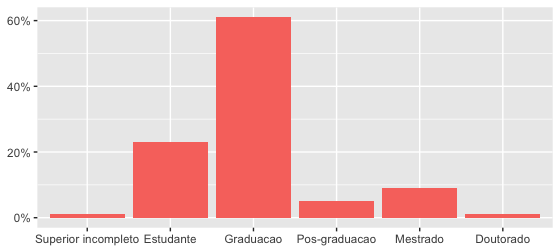
\includegraphics[width=.99\textwidth]{phase2-participants-graduation.png}
  \caption{Distribuição de escolaridade.}
  \label{fig:phase2-participants-graduation}
\end{subfigure}
\begin{subfigure}{.36\textwidth}
  \centering
  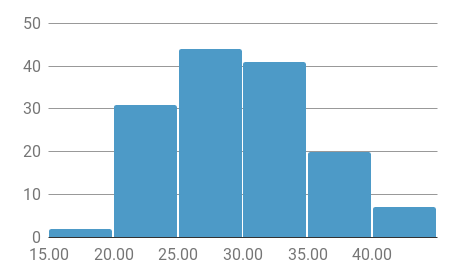
\includegraphics[width=.99\textwidth]{phase2-participants-age.png}
  \caption{Distribuição de idade.}
  \label{fig:phase2-participants-age}
\end{subfigure}% 
\caption{Escolaridade e distribuição de idade dos participantes em S$_2$.}
\label{fig:phase2-participants-graduation-age}
\vspace{-.5cm} 
\end{figure*}

Participaram desta etapa da pesquisa 201 desenvolvedores. 145 respostas vieram da versão em português do questionário e 56 da versão em inglês. Dos participantes, 15\% possuem uma ou mais pós-graduações e 61\% são graduados, esses dados podem ser observados na Figura \ref{fig:phase2-participants-graduation}. A Figura \ref{fig:phase2-participants-age} apresenta o histograma de idade dos participantes, onde podemos observar que tivemos uma abrangência considerável de idade, onde a maior parte possui de 20 a 35 anos.  


Conforme apresentado na Figura \ref{fig:phase2-participants-experience}, 94\% participantes indicaram ter 2 anos ou mais de experiência com desenvolvimento de software e 74\% indicaram 2 anos ou mais de experiência com desenvolvimento Android. Esse resultado nos indica que atingimos desenvolvedores com experiência considerável em desenvolvimento de software e Android. 

\begin{figure*}[!t]
\centering
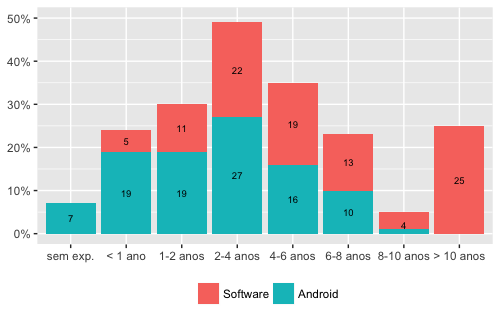
\includegraphics[width=.7\linewidth]{phase2-participants-experience.png}
\caption{Tempo de experiência com desenvolvimento de software e desenvolvimento Android dos participantes de S$_2$.}
\label{fig:phase2-participants-experience}
% \vspace{-.5cm} 
\end{figure*}

\begin{figure*}[!b]
  \centering
  \vspace{-.5cm} 
  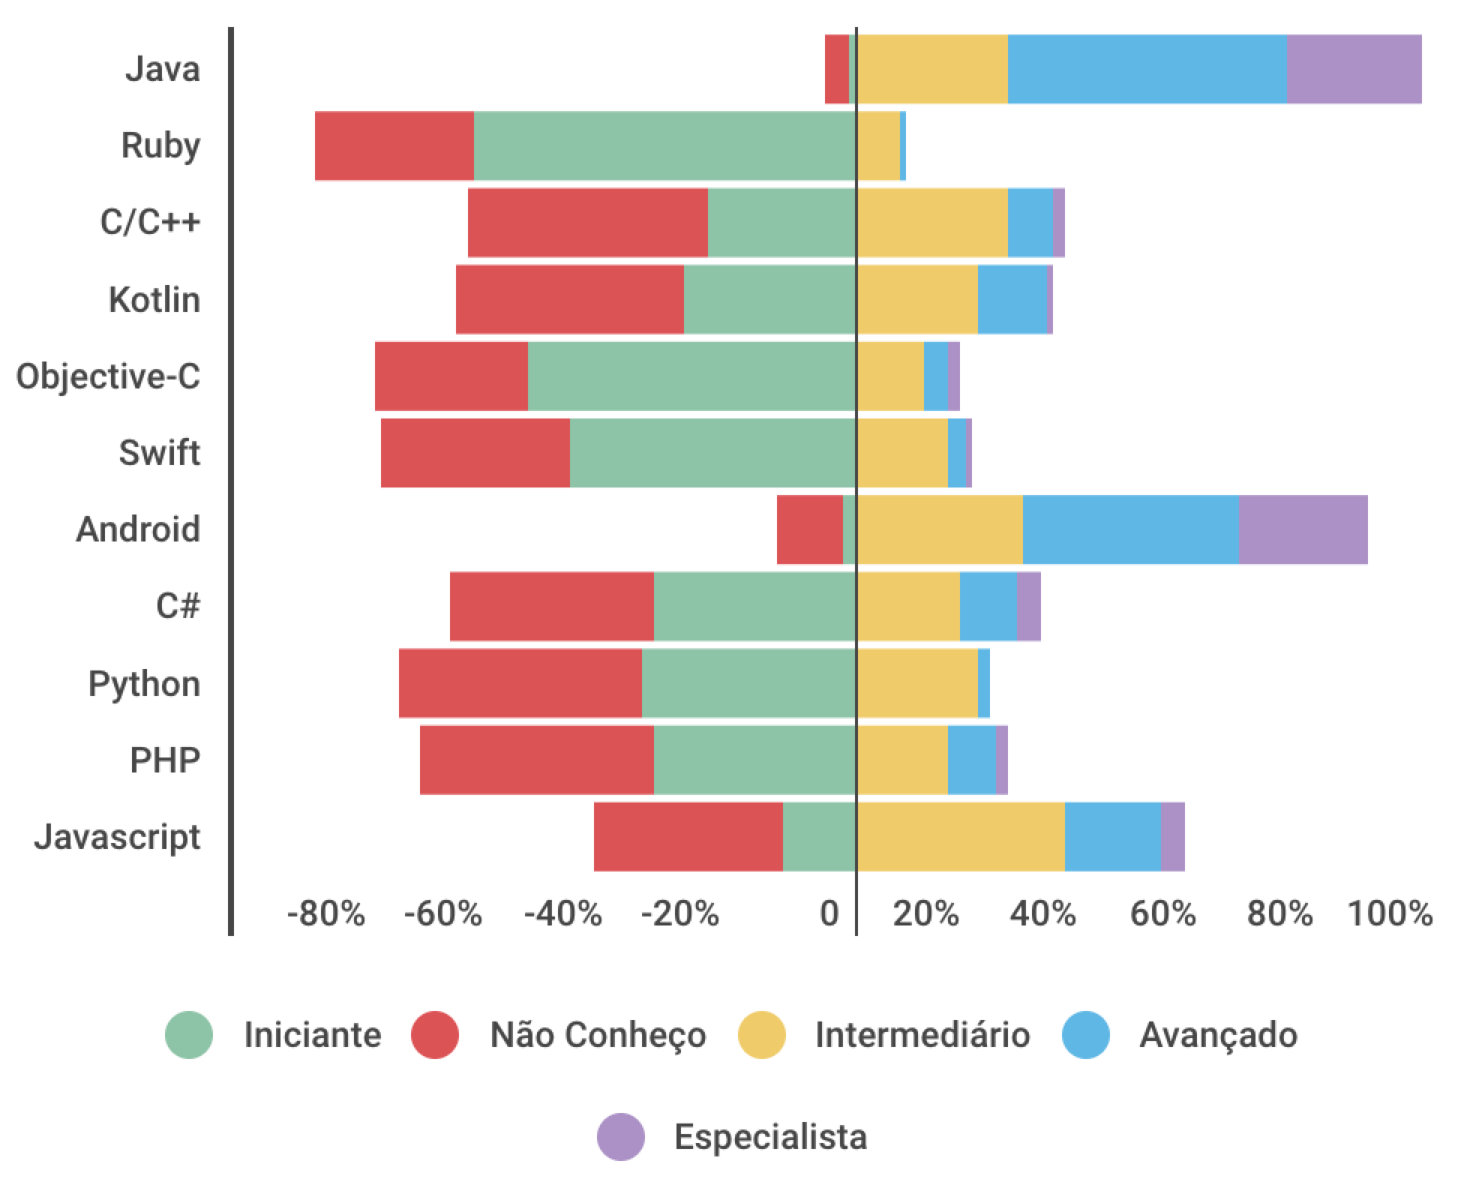
\includegraphics[width=.75\textwidth]{phase2-participants-languages.png}
  \caption{Nível de conhecimento em diversas linguagens de programação orientada a objetos dos participantes de S$_2$.}
  \label{fig:phase2-participants-languages}
  \vspace{-.5cm} 
\end{figure*}

Perguntamos aos desenvolvedores qual seu nível de conhecimento em diversas linguagens orientadas a objetos. Na Figura \ref{fig:phase2-participants-languages} podemos observar que mais de 80\% afirmam ter conhecimento de intermediário a especialista em Java e Android. De 20\% a 58\% dos participantes afirmam ter conhecimento de intermediário a especialista em outras linguagens orientadas a objetos. 5 participantes (2\%) afirmaram não ter conhecimento sobre Android, por este motivo suas respostas foram desconsideradas da análise. 

A Figura \ref{fig:phase2-participants-regions} apresenta a distribuição geográfica global e brasileira dos participantes. Nosso questionário foi respondido por profissionais de 3 continentes e 14 países diferentes porém a maior representatividade dos dados é originada do Brasil, com pouco mais de 78\% dos participantes. Os brasileiros somam 157 profissionais de 18 estados diferentes. Desse total, os estados com maior representatividade foram, na ordem: São Paulo com 57\%, Rio de Janeiro e Minhas Gerais com quase 6\% cada e Rio Grande do Sul com quase 5\%. 10\% dos participantes são originados de países Europeus. Nos Estados Unidos tivemos 2\% provenientes da Califórnia, Pensilvânia, Indiana e Utah e 0,5\% (1 participante) de Ontário no Canadá. \\

\begin{figure*}[!htb]
\centering
\vspace{-.3cm} 
\begin{subfigure}{.52\textwidth}
  \centering
  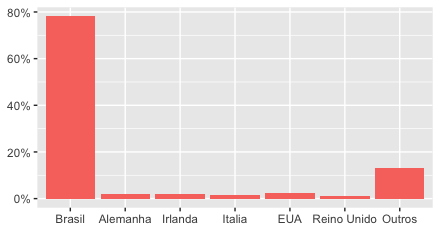
\includegraphics[width=.99\textwidth]{phase-2-participants-region-mundial.png}
  \caption{Distribuição geográfica global.}
  \label{fig:phase2-participants-regions-global}
\end{subfigure}
\begin{subfigure}{.46\textwidth}
  \centering
  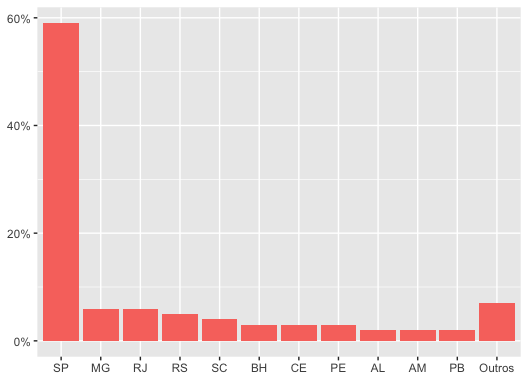
\includegraphics[width=1\textwidth]{phase-2-participants-region-brasil.png}
  \caption{Distribuição geográfica brasileira.}
  \label{fig:phase2-participants-regions-brasil}
\end{subfigure}% 
\caption{Distribuição geográfica global e brasileira dos participantes de S$_2$.}
\label{fig:phase2-participants-regions}
% \vspace{-.5cm} 
\end{figure*}

Podemos concluir que tivemos certa abrangência geográfica, porém o padrão geográfico obtido em S$_1$ se repetiu em S$_2$, e apesar de termos tido certa abrangência global, a maior representatividade é proveniente do Brasil, logo, continuamos acreditando que o mais apropriado seja dizer que a percepção de frequência e importância dos maus cheiros propostos representam a opinião de desenvolvedores brasileiros, principalmente de São Paulo.


\subsubsection{Análise dos Dados}
\label{etapa-2-analise}

Para análise dos dados, as opções das escalas \textit{likert} de \textbf{\small frequência} e \textbf{\small importância} foram codificadas em números de 1 a 5. Por exemplo, as opções ``Nunca'' (da escala de frequência) e ``Não é importante'' (da escala de importância) foram codificadas com 1, as opções ``Raramente'' (frequência) e ``Pouco importante'' (importância) com 2, e assim sucessivamente até as opções ``Muito frequente'' (frequência) e ``Muito importante'' (importância) que foram codificadas com~5.

De modo a avaliar a percepção dos desenvolvedores Android sobre a frequência e importância dos maus cheiros propostos, para análise dos dados extraímos de cada afirmação a mediana, moda e desvio padrão. Para os maus cheiros que apresentamos mais de uma afirmação, extraímos a média desses dados para representá-los. Por exemplo, foram apresentadas três afirmações de frequência sobre o mau cheiro \textsc{\small Comportamento Suspeito}, a moda que o representa é a média das modas de cada afirmação, que neste caso foi $(3 + 4 + 4) \div 3 = 3,7 \approx 4$.

De modo a avaliar quais maus cheiros são considerados frequentes realizamos uma simplificação da escala \textit{likert} de \textbf{\small frequência}. Classificamos de \textbf{\small frequência baixa} as resposta ``Raramente'', de \textbf{\small frequência moderada} as respostas ``Às vezes'' e por último, classificamos de \textbf{\small frequência alta} as respostas ``Frequente'' e ``Muito frequente''. Não obtivemos nenhuma afirmação com moda (MO) igual 1, ou seja, ``Nunca'', e por isso não criamos uma classificação para ela.

De modo similar, para avaliar quais maus cheiros são considerados importantes, também realizamos uma simplificação da escala \textit{likert} de \textbf{\small importância}. Classificamos de \textbf{\small importância baixa} as resposta ``Pouco importante'', de \textbf{\small importância moderada} as respostas ``Razoavelmente importante'' e classificamos de \textbf{\small importância alta} as respostas de ``Importante'' e ``Muito importante''. Também não foi necessário criar uma classificação para respostas ``Não é importante'' pois nenhuma das afirmações obteve MO igual a 1.















\subsection[Etapa 3 - Percepção de Desenvolvedores sobre os Maus Cheiros]{Etapa 3 - Percepção de Desenvolvedores sobre os Maus Cheiros Android}
\label{etapa-3}

Para responder a S$_3$ validamos a percepção de desenvolvedores Android sobre códigos afetados por 7 maus cheiros, os considerados mais frequentes (vide Tabela \ref{tab:selected-smells}) pelos respondentes de S$_2$. Os dados foram coletados por meio de um experimento de código online (S$_3$) onde cada participante foi solicitado a avaliar a qualidade de 6 códigos-fontes relativos à camada de apresentação Android. Recebemos 70 respostas. Vale ressaltar que esse experimento já foi realizado em pesquisas similares, como as de Aniche et al. \cite{AnicheSmellsMVC:17, MvcSmells:16} e Palomba et al. \cite{Palomba_Do_2014}, com o mesmo objetivo de validar a percepção de desenvolvedores sobre maus cheiros de código.  


Nossos resultados confirmam estatisticamente que desenvolvedores Android percebem 6 dos 7 maus cheiros avaliados. Não obtivemos dados suficientes para tirar conclusões estatísticas sobre um dos maus cheiros. A seguir, na Seção \ref{etapa-3-experimento}, apresentamos detalhes sobre o experimento e na Seção \ref{etapa-3-participantes-analise}, detalhes sobre os participantes e como realizamos a análise dos dados. Os resultados desta etapa podem ser conferidos na Seção~\ref{phase3-results}.


\subsubsection{Experimento}
\label{etapa-3-experimento}

O questionário do experimento foi elaborado no idioma português, divulgado em redes sociais como Twitter e LinkedIn e o grupo do Slack Android Dev Br\footnote{http://slack.androiddevbr.org} e esteve disponível por 1 mês. No cabeçalho informamos que o experimento fazia parte de uma pesquisa sobre qualidade de código Android e que os dados fornecidos poderiam futuramente ser publicados de forma anônima. 

O experimento continha duas seções principais ambas com todas as perguntas sendo opcionais. A primeira seção teve como objetivo coletar informações demográficas, principalmente com relação à experiência dos participantes. Na segunda seção os participantes foram solicitados a analisar 6 códigos-fontes, 4 \textbf{\small \textit{``mau cheirosos''}}, ou seja, afetados por um dos maus cheiros avaliados, e 2 \textbf{\small \textit{``limpos''}}, ou seja, não afetado pelos maus cheiros avaliados. Para cada código, o participante também foi solicitado a responder as seguintes perguntas:

\noindent 
\begin{itemize}
  \item[P1] Na sua opinião, este código apresenta algum problema de design e/ou implementação? (SIM/NÃO)
  \item[P2] Se SIM, por favor explique quais são, na sua opinião, os problemas que afetam este código. (Pergunta aberta)
  \item[P3] Se SIM, por favor avalie a severidade do problema de design e/ou implementação selecionando dentre as opções a seguir. (Escala \textit{Likert} de 5 pontos de 1, muito baixa, até 5, muito alta).
\end{itemize}

Segundo Fink (1995) \cite{Fink:95}, o tamanho da amostra se refere ao número de respondentes necessários para que os resultados obtidos sejam precisos e confiáveis, e que o aumento no tamanho da amostra diminui o erro. Moscarola (1990) \cite{Moscarola:90} resume essa ideia com ``\textit{a lei dos grandes números}'', segundo a qual ele argumenta que ``\textit{com uma amostra inferior a 30 observações se tem chances de encontrar tanto um valor errôneo ou defasado como um valor se aproximando da realidade}''. Sendo assim, para termos maior confiabilidade sobre os resultados, objetivamos coletar em média 30 pontos por mau cheiro avaliado. Isso significa cada mau cheiro ter em média 30 desenvolvedores avaliando um código afetado por ele. Portanto, o cálculo necessário para obter o número total de participantes necessários para avaliar todos os maus cheiros é (MC remete a Mau Cheiro): 

\begin{center}
  $(MC_{total} \times MC_{pontos}) \div MC_{avaliados}$
\end{center}

Onde $MC_{total}$ indica o total de maus cheiros a serem avaliados, $MC_{pontos}$ indica o total de pontos que se deseja obter para cada mau cheiro e $MC_{avaliados}$ indica o total de maus cheiros avaliados por cada participante, ou seja, quantos códigos mau cheirosos serão apresentados, que no nosso caso são 4. Aplicando esse cálculo ao nosso contexto, concluímos que seriam necessários aproximadamente 150 participantes:

\begin{center}
  $(20 \times 30) \div 4 = 150$
\end{center}
 
Visto que este experimento exige um esforço maior dos participantes (analisar 6 códigos-fontes) optamos por iniciá-lo com um subconjunto menor de maus cheiros objetivando obter 30 pontos por mau cheiro rapidamente. 

Iniciamos o experimento com 7 maus cheiros, considerados mais frequentes (maior somatória de frequência alta e moderada), conforme apresentamos na Tabela \ref{tab:selected-smells}. Entendemos que este foco agrega mais valor do que focar nos mais importantes pois, segundo Taibi et al. \cite{Taibi:17} apesar de alguns maus cheiros serem considerados na teoria muito críticos por desenvolvedores, na prática eles são mais toleráveis. O experimento foi elaborado de modo que, conforme um mau cheiro alcançasse os 30 pontos, era possível substituí-lo ou mesmo removê-lo do experimento.



\begin{table}
\centering
\renewcommand*{\arraystretch}{1}
\footnotesize 
\caption{Sete maus cheiros avaliados no experimento de código sobre a percepção de desenvolvedores Android.}
\begin{tabular}{@{}lp{7cm}c@{}}
\toprule
\# & \multirow{1}{*}{\textbf{Mau Cheiro}} & \multirow{1}{*}{\textbf{Frequência Alta + Moderada}}  \\
\toprule
1 & \textsc{\small Longo Recurso de Estilo}          & 74.38\% \\
2 & \textsc{\small Adapter Complexo}                 & 70.65\% \\
3 & \textsc{\small Componente de UI Acoplado}        & 69.65\% \\
4 & \textsc{\small Layout Profundamente Aninhado}    & 66.67\% \\
5 & \textsc{\small Componente de UI Cérebro}         & 66.67\% \\
6 & \textsc{\small Atributos de Estilo Repetidos}    & 65.92\% \\
7 & \textsc{\small Comportamento Suspeito}           & 65.67\% \\
\bottomrule
\end{tabular}
\label{tab:selected-smells}
\end{table}


Os 6 códigos apresentados foram randomicamente selecionados de um conjunto de 50 códigos. Esse conjunto foi composto por 35 códigos mau cheirosos (cinco para cada mau cheiro avaliado) e 15 códigos limpos. Vale salientar que, para mitigar possíveis vieses de confundimento, nos dois grupos de códigos (mau cheirosos e limpos) selecionamos apenas \textit{Activities}, \textit{Fragments}, \textit{Adapters}, \textit{Listeners}, recursos de \textit{Layout}, \textit{String} e \textit{Style}, uma vez que são esses os elementos da camada de apresentação Android, cujo os maus cheiros propostos e avaliados tratam.

\begin{table}
\centering
\renewcommand*{\arraystretch}{1}
\footnotesize
\caption{Listagem dos nove projetos de software livre Android utilizados para coletar os códigos do experimento.} 
\begin{tabular}{@{}p{9cm}lll@{}}
\toprule
\multirow{2}{*}{\textbf{Código-Fonte}} & \multicolumn{3}{c}{\textbf{Google Play Store}} \\ \cmidrule{2-4}
                                       & \textbf{Estrelas}    & \textbf{Instalações}    & \textbf{Versão} \\
\bottomrule
https://github.com/uberspot/2048-android & 4.2 &  1.000.000 - 5.000.000 & 2.08 \\
https://github.com/jereksel/Bucket & 4.2 &  1.000 - 5.000 & 0.2.1-play \\
https://github.com/TeamAmaze/AmazeFileManager & 4.3 &  500.000 - 1.000.000 & 3.2.1 \\
https://gitlab.com/cfabio/AltcoinPrices &  &   &  \\
https://github.com/pinetum/AirUnlock-for-Android &  &   &  \\
https://github.com/SecUSo/privacy-friendly-weather & 3.8 &  1.000 - 5.000 & 1.1 \\
https://github.com/Xlythe/Calculator &  &   &  \\
https://github.com/mkulesh/microMathematics & 4.7 &  500 - 1.000 & 2.15.6 \\
https://github.com/openfoodfacts/openfoodfacts-androidapp & 4.0 &  1.000 - 5.000 & 0.7.4 \\
\bottomrule
\end{tabular}
\label{tab:android-projects}
\end{table}

Os códigos utilizados no experimento foram extraídos de projetos de software livre Android selecionados aleatoriamente do repositório F-Droid\footnote{f-droid.org é um repositório que lista projetos gratuitos e software livre Android (FOOS, do inglês \textit{Free and Open Source Software}).}. A Tabela \ref{tab:android-projects} apresenta esses projetos, bem como informações sobre avaliação (estrelas), total de instalações e versão atual do aplicativo na Google Play Store, loja oficial de aplicativos Android, para os aplicativos que lá estão disponíveis. 


A seleção dos códigos foi feita de forma manual, pois como os maus cheiros estão sendo propostos nesta pesquisa, ainda não existem heurísticas definidas ou ferramentas que os detectem automaticamente em projetos Android. Para cada mau cheiro a ser avaliado, buscamos nos projetos pelo tipo de código que poderia ser afetado por ele. Por exemplo, o mau cheiro \textsc{\small Atributos de Estilo Repetidos} pode afetar recursos de \textit{Layout} ou \textit{Style}, mas não \textit{Activities}, deste modo, para encontrar códigos afetados por ele, buscamos nos projetos por recursos de \textit{Layout} ou \textit{Style}. Após encontrado, o código era analisado de modo a verificar se apresentava algum dos sintomas do mau cheiro (o catálogo com a definição dos sintomas dos maus cheiros Android pode ser conferido na Seção \ref{phase1-code-smells-derivation}). Caso o código apresentasse o sintoma, ele era separado para ser usado no experimento. 

Repetimos esse procedimento para cada mau cheiro a ser avaliado, passando por cada um dos projetos selecionados. Quando não encontrávamos códigos nos projetos já selecionados, selecionávamos aleatoriamente outro projeto e repetíamos a busca pelo mau cheiro. Deste modo, 9 projetos foram necessários para encontrarmos códigos exemplos, maus cheirosos e limpos, para os 7 maus cheiros.


Para cada código separado para o experimento, foi criado um \textit{gist}\footnote{\textit{Gist} é uma forma de compartilhar conteúdo, inclusive trechos de código, pela plataforma GitHub \cite{Gists}.}. A lista com todos os \textit{gists} pode ser conferida no Apêndice \ref{experiment-gists}. Pequenas modificações foram feitas nos códigos com o objetivo de reduzir o esforço cognitivo do participante ao ler o código-fonte apresentado e isolar o mau cheiro a ser avaliado. Desse modo, reduzimos o esforço cognitivo através da remoção de declarações de \textit{packages}, \textit{imports} e comentários. Para isolar o mau cheiro, diversas e variadas pequenas mudanças foram realizadas a depender do código e do mau cheiro a ser isolado. Deste modo, cada \textit{gist} com código mau cheiroso, apresentava apenas um dos maus cheiros avaliados. 

Para mitigar possíveis viés de seleção, foram criados cinco \textit{gists} diferentes para cada mau cheiro, totalizando 35 \textit{gists} mau cheirosos diferentes. Sobre os \textit{gists} com códigos limpos, selecionamos cinco códigos de componentes da camada de apresentação Android, dentre eles \textit{Activities}, \textit{Fragments}, \textit{Adapters} e \textit{Listeners}, cinco recursos de \textit{Layout} e cinco recursos de \textit{Style}, totalizando 15 \textit{gists} de códigos limpos. Nenhum dos maus cheiros avaliados afetava recursos de \textit{String} ou \textit{Drawables}, e por este motivo não foram selecionados códigos desses~tipos.

Para reduzir efeitos de aprendizagem e viés de ordem, cada participante recebeu os seis códigos randomicamente selecionados, em ordem aleatória. Como nossas necessidades para o experimento eram bem peculiares, foi desenvolvido um software específico\footnote{Repositório do software desenvolvido para aplicação do experimento de código: github.com/suelengc/code-experiment-survey-app} para aplicá-lo. Além disso, os participantes não foram informados de quais códigos pertenciam a quais grupos (maus cheirosos ou limpos). Os participantes foram informados apenas de que a pesquisa tinha como objetivo estudar a qualidade de códigos da camada de apresentação de aplicativos Android nativos. Não foi imposto nenhum limite de tempo para completar a tarefa.

Durante o tempo em que o experimento esteve aberto, de 05 de Dezembro à 5 de Janeiro, obtivemos respostas suficientes para avaliar os 7 maus cheiros lançados inicialmente.


\subsubsection{Participantes e Análise dos Dados}
\label{etapa-3-participantes-analise}

Participaram desta etapa da pesquisa 70 desenvolvedores. Dos participantes, 82\% possui 2 anos ou mais de experiência com desenvolvimento de software e 52\% possui 2 anos ou mais de experiência com desenvolvimento Android. Das 70 respostas, 14 foram desconsideradas ou pelo desenvolvedor não ter experiência com desenvolvimento Android (11\%) ou ter respondido não à pergunta ``\textit{Na sua opinião, este código apresenta algum problema de design e/ou implementação?}'' para todos os 6 códigos apresentados. Estes dados podem ser observados na Figura \ref{fig:phase3-participants-experience}. Perguntamos aos participantes quantos aplicativos Android nativo eles já haviam publicado, 55\% dos participantes afirmam ter publicado pelo menos um aplicativo, destes, 25\% afirmam já terem publicado mais de cinco aplicativos.


\begin{figure*}[!b]
\centering
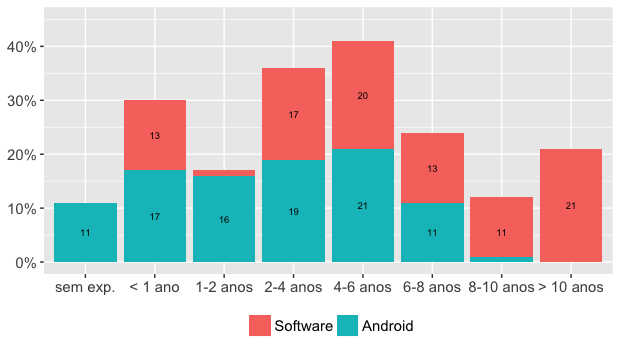
\includegraphics[width=.7\linewidth]{phase3-participants-experience2.png}
\caption{Tempo de experiência com desenvolvimento de software e desenvolvimento Android dos participantes de S$_3$.}
\label{fig:phase3-participants-experience}
\vspace{-.5cm} 
\end{figure*}

Para comparar as distribuições de severidade para os dois grupos de códigos (mau cheirosos e limpos), utilizamos o teste não pareado de Mann-Whitney \cite{Conover:99}. Esse teste é usado para analisar a significância estatística das diferenças entre a severidade atribuída pelos respondentes aos problemas que eles observaram nos códigos. Os resultados são considerados estatisticamente significativos em ``valor p'' ou $\alpha \leq$  0,05. Também estimamos a magnitude das diferenças usando o Delta de Cliff (\textit{d}), uma medida de tamanho de efeito não paramétrico \cite{EffectSize:05} para dados ordinais. Seguimos diretrizes bem estabelecidas \cite{EffectSize:05} para interpretar os valores do tamanho do efeito, sendo: desprezível para | \textit{d} | < 0,14, pequeno para 0,14 $\leq$ | \textit{d} | < 0,33, médio para 0,33 $\leq$ | \textit{d} | < 0.474, e grande para | \textit{d} | $\geq$ 0,474. Finalmente, relatamos resultados qualitativos derivados das respostas abertas dos participantes.

Para medir a significância estatística das diferenças, comparamos as severidades dos códigos mau cheirosos às severidades dos códigos limpos. Os códigos limpos foram segmentados em três grupos: componentes limpos, ou seja, \textit{Activities}, \textit{Fragments}, \textit{Adapters} ou \textit{Listeners} limpos, recursos de \textit{style} limpos e recursos de \textit{layout} limpos. As severidades dos maus cheiros que afetam componentes, ou seja: \textsc{\small Componente de UI Cérebro}, \textsc{\small Componente de UI Acoplado}, \textsc{\small Adapter Complexo} e \textsc{\small Comportamento Suspeito}, foram comparadas às severidades do grupo de componentes limpos. 

As severidades dos maus cheiros que afetam recursos de \textit{layout}, ou seja: \textsc{\small Layout Profundamente Aninhado} e \textsc{\small Atributos de Estilo Repetidos} foram comparada às severidades do grupo de recursos de \textit{layout} limpos. As severidades dos maus cheiros que afetam recursos de \textit{style}, ou seja: \textsc{\small Longo Recurso de Estilo} e \textsc{\small Atributos de Estilo Repetidos} foram comparadas com às severidades do grupo de recursos de \textit{style} limpos.

Fizemos também duas análises consolidativas. Uma consolidou a percepção sobre maus cheiros que afetam componentes Android, ou seja, comparamos as severidades de todos os maus cheiros que afetam componentes da camada de apresentação Android com componentes limpos. De modo similar, consolidamos a percepção sobre maus cheiros que afetam recursos Android, comparando as severidades de todos os maus cheiros que afetam recursos às severidades dos grupos de recursos de \textit{layout} e \textit{style} limpos.




% -*- root: dissertation.tex -*-
\subsection{Ameaças à Validade}
\label{ameacas}

Nesta seção, apresentamos as ameaças à validade seguindo os critérios de validade definidos por Claes et al. \cite{Wohlin:00}.

% conclusão
As ameaças à \textit{validade de conclusão} dizem respeito à relação entre o tratamento e o resultado. Embora este seja principalmente um estudo observacional, sempre que possível, utilizamos um suporte apropriado de procedimentos estatísticos, integrados com medidas de tamanho de efeito que, além da significância das diferenças encontradas, destacam a magnitude de tais diferenças. 

% interna
As ameaças à \textit{validade interna} dizem respeito a fatores externos que não consideramos que possam afetar as variáveis e as relações que estão sendo investigadas. Utilizamos escalas padrões de importância e frequência em S$_2$, mesmo não tendo uma opção neutra, para caso o participante não soubesse opinar sobre alguma afirmação. Apesar de ser possível utilizar outras escalas, até o momento não encontramos nenhuma pesquisa sobre qual escala é mais apropriada para o contexto de validar a importância e frequência de maus cheiros. De modo a mitigar esse problema, o processo de preparação de S$_2$ incluiu a validação com 2 desenvolvedores experientes e 2 testes piloto.

Na literatura, maus cheiros são derivados do conhecimento empírico de desenvolvedores experientes \cite{Refactoring:99, Riel:96, CleanCode:08, Webster:95}. Pesquisas também mostraram que a experiência e conhecimento desempenham um importante papel na percepção de maus cheiros \cite{Palomba_Do_2014, Taibi:17}. Embora não tenhamos restringido nenhum dos questionários (S$_1$ e S$_2$) ou experimento (S$_3$) a desenvolvedores com determinado tempo de experiência, todos eles possuíam perguntas que nos possibilitou avaliar a experiência dos respondentes. Por fim, obtivemos a maioria das respostas de desenvolvedores com 2 anos ou mais de experiência em desenvolvimento de software e Android.

Não controlamos se um participante de uma etapa da pesquisa participou de outra, deste modo, não podemos ignorar possíveis vieses de participantes recorrentes. Entretanto, ambos os questionários e experimento eram independentes e não faziam qualquer referência um ao outro.

Também é possível que imprecisões ocorram devido a algum erro de implementação no sistema desenvolvido por nós para o experimento de código. Para mitigar esse risco, nosso sistema foi desenvolvido com base no sistema de software livre desenvolvido por Aniche et al. \cite{AnicheSmellsMVC:17, MvcSmells:16} para validar a percepção de maus cheiros relacionados ao arcabouço Spring MVC. 

Embora nossa pesquisa tenha sido realizada em três etapas, estamos cientes que os dados foram todos coletados por questionários online, podendo trazer imprecisões devido ao uso de um único meio de coleta de dados. Para mitigar esse problema, nossas etapas se basearam em metodologias já usadas em outras pesquisas similares e também realizamos validações e testes piloto antes de lançarmos os questionários. 

% constructo
As ameaças à \textit{validade do constructo} dizem respeito à relação entre a teoria e a observação, e neste trabalho são principalmente devido à codificação realizada. Uma vez que a codificação das respostas de S$_1$ foi realizada apenas pelo autor, estamos cientes que imprecisões podem ser introduzidas. Para mitigar esse problema, validamos por meio de S$_2$, que os sintomas extraídos são considerados frequentes e importantes por desenvolvedores Android. Vale lembrar que o processo de preparação de S$_2$ incluiu duas validações com desenvolvedores experientes e dois pilotos. Além disso, os dados usados para a codificação, bem como as categorias derivadas estão disponíveis para inspeção no apêndice online \cite{apendice}.

A seleção dos códigos usados em S$_3$ foi feita manualmente buscando pelos sintomas dos maus cheiros detalhados na seção \ref{phase1-code-smells-derivation}. Podem haver melhores maneiras de proceder com essa seleção. Pesquisas adicionais precisam ser conduzidas para otimizar esse processo. No entanto, nossa seleção atual foi capaz de detectar códigos percebidos como problemáticos pelos desenvolvedores. Entretanto, estamos cientes de que essa seleção manual pode introduzir imprecisões. De modo a mitigá-las, selecionamos cinco diferentes códigos maus cheirosos para cada mau cheiro analisado e cinco diferentes códigos para cada componente Android e recursos de \textit{style} e \textit{layout}. 

% externa
As ameaças à \textit{validade externa} referem-se à generalização dos resultados. Definimos como camada de apresentação os oito elementos aqui pesquisados. Embora essa definição tenha sido embasada na documentação oficial, sabemos que existem recursos não investigados e podem haver classes menos comumente usadas também não avaliadas que de alguma forma se relacionem também à camada de apresentação. Logo, não afirmamos que camada de apresentação se limita apenas aos oito elementos aqui estudados.

Validamos com sucesso a percepção de forma negativa de 6 maus cheiros com desenvolvedores Android por meio de um experimento de código online. Embora este experimento tenha sido usado em outras pesquisas similares com o mesmo objetivo \cite{AnicheSmellsMVC:17, MvcSmells:16, Palomba_Do_2014} e tenhamos obtido pontos por mau cheiro suficientes para ter confiabilidade estatística, não afirmamos que todo desenvolvedor Android irá perceber os maus cheiros validados. 

Embora tenhamos tido certa abrangência geográfica nas respostas de S$_1$ e S$_2$, nossos resultados foram majoritariamente de brasileiros, principalmente de São Paulo. Logo, não afirmamos que nossos resultados são generalizáveis globalmente. Mais pesquisas precisam ser conduzidas neste sentido para verificar a validade dos maus cheiros por desenvolvedores de outras regiões. 

Nosso catálogo é composto de 20 maus cheiros na camada de apresentação Android. Entretanto, coletamos poucas respostas em S$_1$ e deste modo, não afirmamos que este é um catálogo abrangente ou mesmo completo. Pesquisas adicionais são necessárias para investigar outras possíveis más práticas na camada de apresentação de aplicativos Android e mesmo validar se os maus cheiros aqui definidos, porém não validados, são realmente percebidos e relevantes. 

